\subsection{Standard Model Single Top}
\label{sec:Bkg:SingleTop}

Standard Model single top consists of 3 to 7 percent of the background in any one $\RISR$ bin. In total, single top consist of 4 percent of the total background in SRC.  A 1 lepton single top control region is defined in section \ref{sec:SingleTopCR}.  The single top CR is orthogonal to both the $W$+jets control region and ttbar control region.  \\

\subsubsection{Single Top Control Region}
\label{sec:SingleTopCR}

\begin{table}[htpb]
  \caption{Selection for the 1-lepton, single top control region. The signal lepton is treated as a jet for the jet counting and \pt\ ordering as well as for the top reco.}
  \begin{center}
    \begin{tabular}{c|c}
      \hline \hline
 	& CRST           \\ \hline
      Number of leptons             & 1                                            \\ 
      Number of jets (incl. lepton) & $\geq 4$                                     \\ 
      $\pt$ of jets (incl. lepton)  & (80,80,40,40) GeV                            \\ 
      \mindphijettwomet             & $> 0.4$                                      \\ \
      $\met$                        & $>250$ GeV                                   \\ \hline
      \mtlepmet                     & $>30$,$<100$ GeV \\ 
      Number of $b$-jets            & $\ge2$                          \\ 
      \mantikttwelvezero            & v$>120$ GeV       \\
      \mtbmin                       & $>200\,$GeV   \\ 
      \mindrblep                    & $>2.0$             \\ 
      \drbjetbjet                   & $>1.5$               \\ \hline \hline
    \end{tabular}
  \end{center}
  \label{tab:1LCR_BaseDefs}
\end{table}

The selection on $\Delta R(b_{0,1},\ell)_{\mathrm{min}}$, defined as the minimum $\Delta R$ between the two jets with the highest b-tag weight and the selected lepton, ensures the orthogonality of CRTop and CRST. In CRST the requirement on the $\Delta R$ of the two leading-weight b-jets is necessary to reject a large part of the remaining \ttbar\ background and reach a single top purity of $\sim$50\%. \\
Data-MC comparisons in the single top control region are shown in Table~\ref{tab:CRST} and for a selection of variables are shown in Fig.~\ref{fig:CRST},~\ref{fig:CRSTPTs}, and~\ref{fig:CRSTMasses}. \\

\begin{table}[!htb]
  \centering
  \begin{tabular}{c|c}
\hline\hline
\multicolumn{2}{c}{\bf CRST (44\% purity)} \\ \hline 
Z & 0.11 $\pm$ 0.05 \\
dibosons & 1.52 $\pm$ 0.54 \\
ttbar & 34.17 $\pm$ 2.10 \\
singleTop & 45.62 $\pm$ 1.41 \\
ttV & 2.42 $\pm$ 0.19 \\
W & 19.72 $\pm$ 1.69 \\
\hline
Total MC & 103.57 $\pm$ 3.10 \\
Data & 113.00 $\pm$ 10.63 \\
 \hline
SF & 1.21 $\pm$ 0.29 \\
\hline\hline
\end{tabular}

  \caption{Yields in the CRST in \intlumi\ \ifb\ of data.  }
  \label{tab:CRST}
\end{table}

\begin{figure}[htbp]
\begin{center}
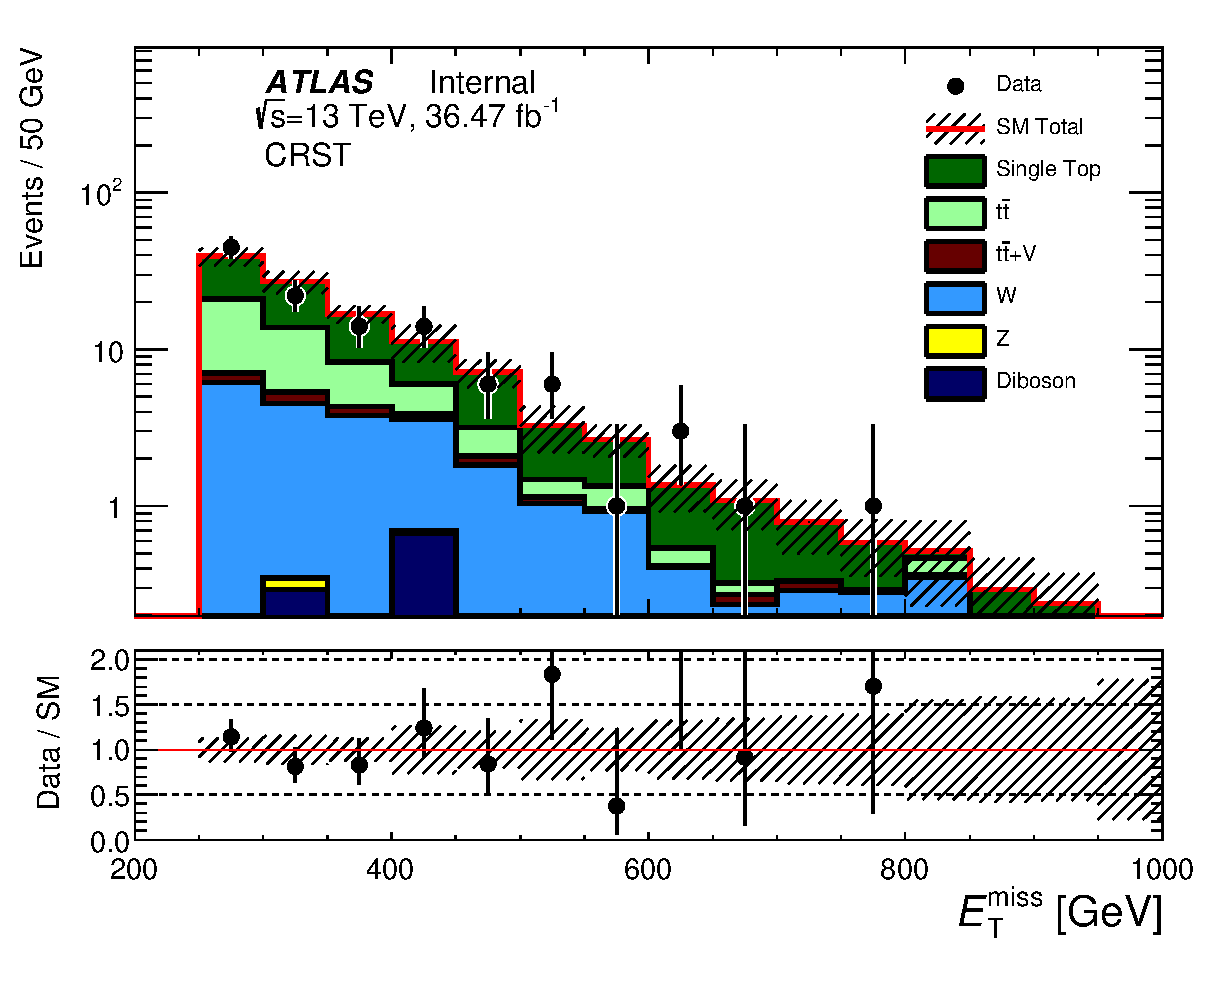
\includegraphics[width=0.45\textwidth]{figures/singleTop/postfit/Met_CRST_log.eps}
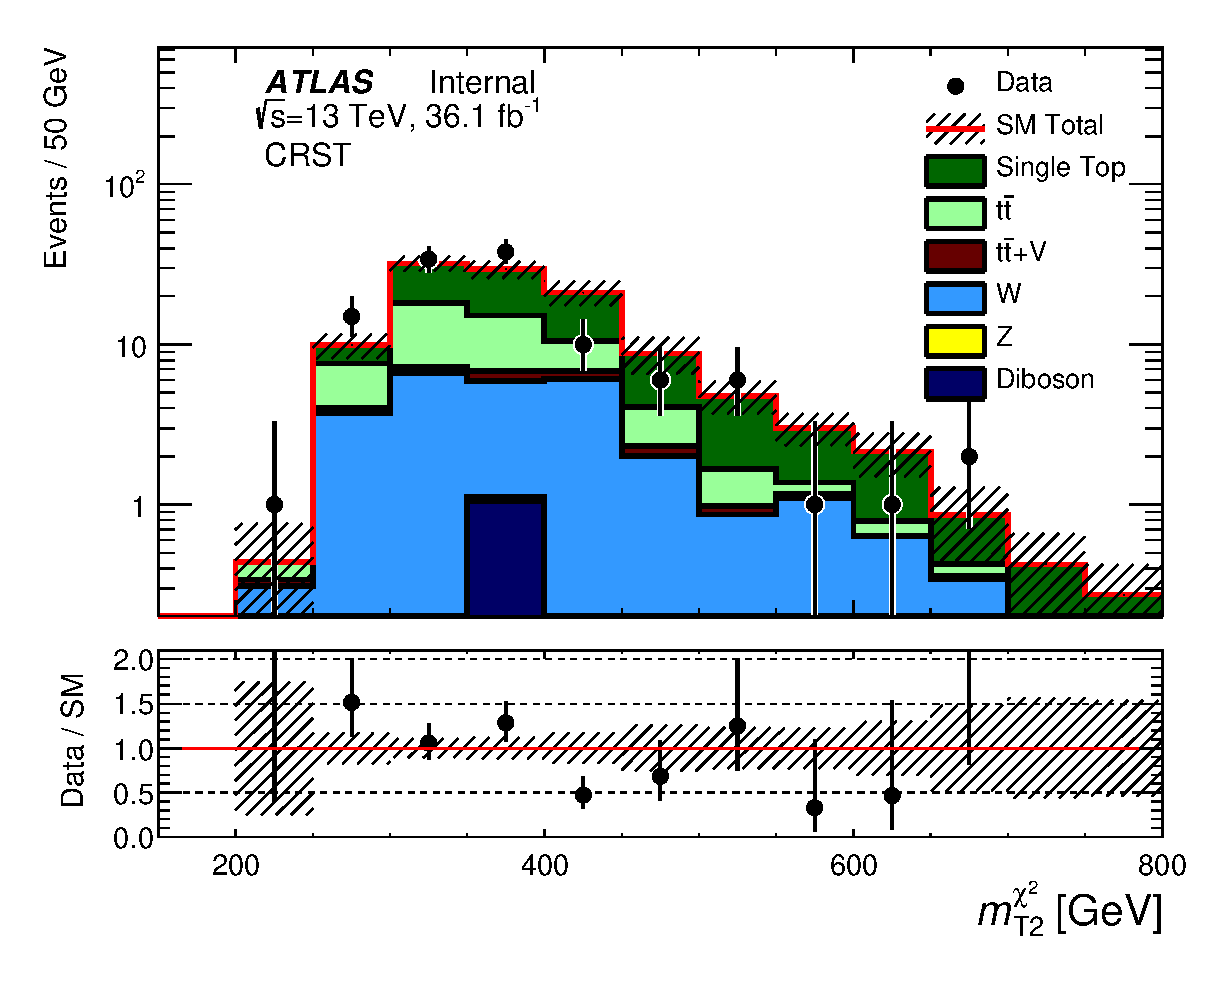
\includegraphics[width=0.45\textwidth]{figures/singleTop/postfit/MT2Chi2_CRST_log.eps}
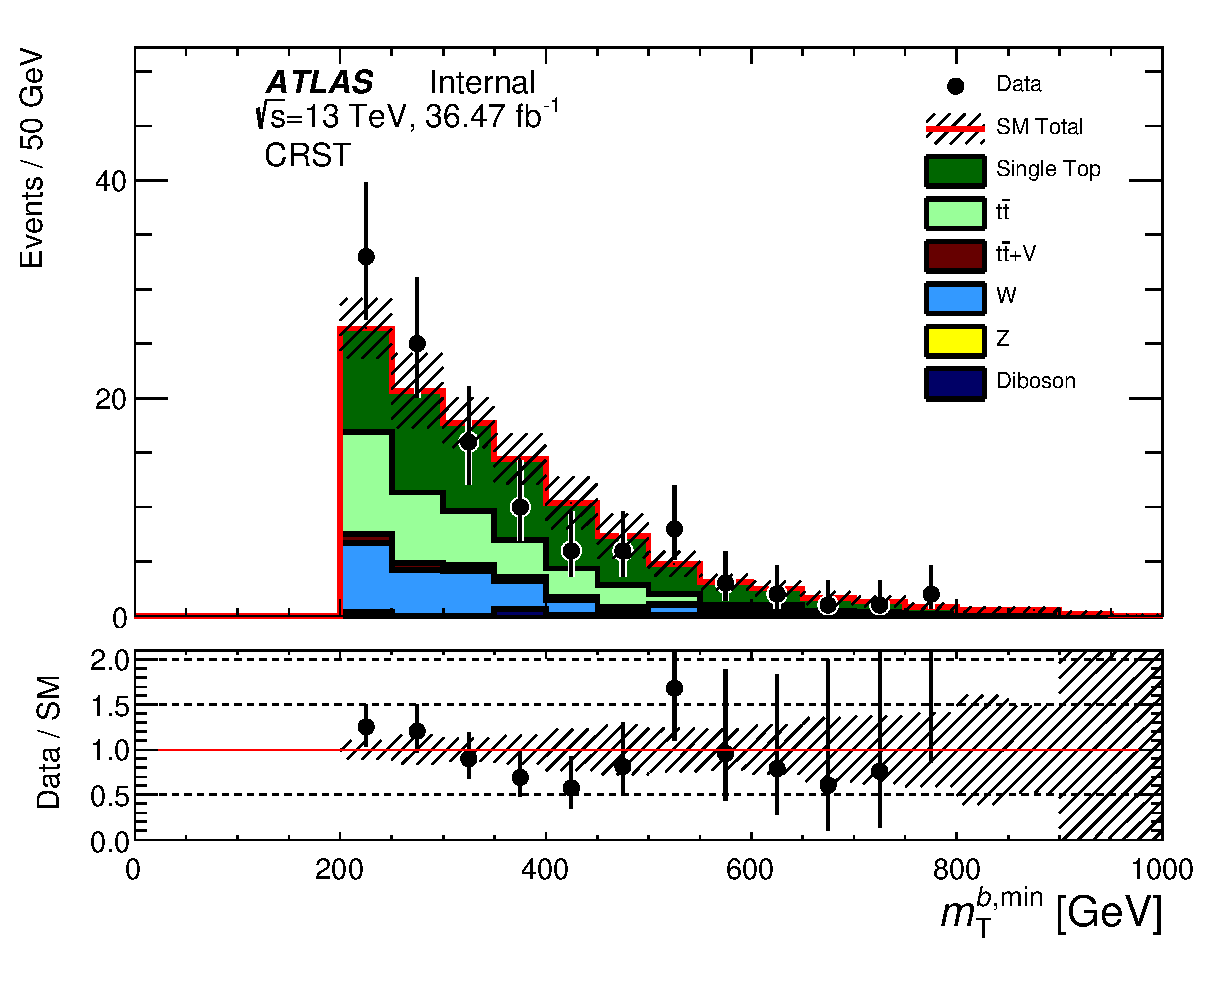
\includegraphics[width=0.45\textwidth]{figures/singleTop/postfit/MtBMin_CRST.eps}
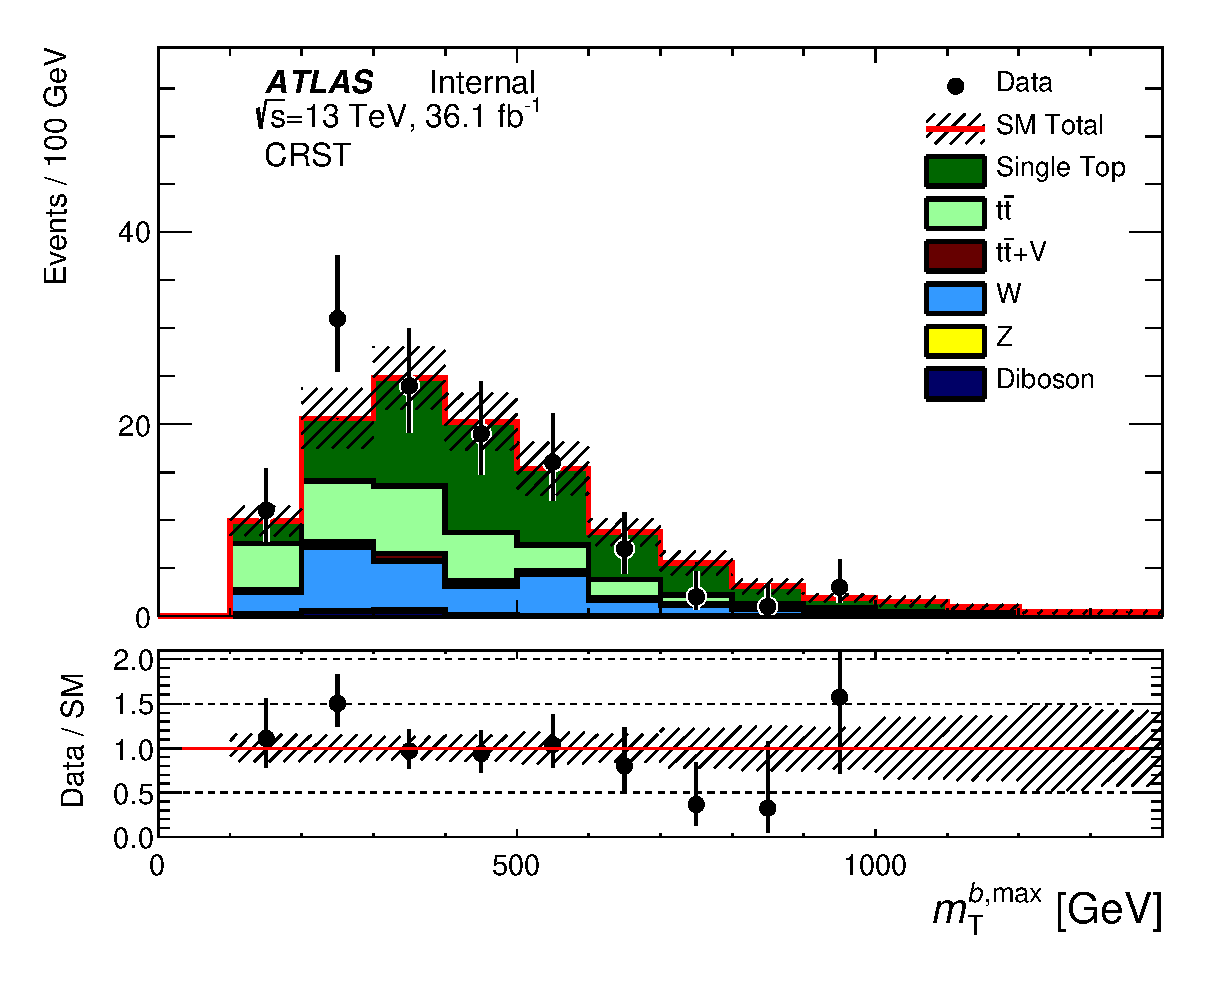
\includegraphics[width=0.45\textwidth]{figures/singleTop/postfit/MtBMax_CRST.eps}
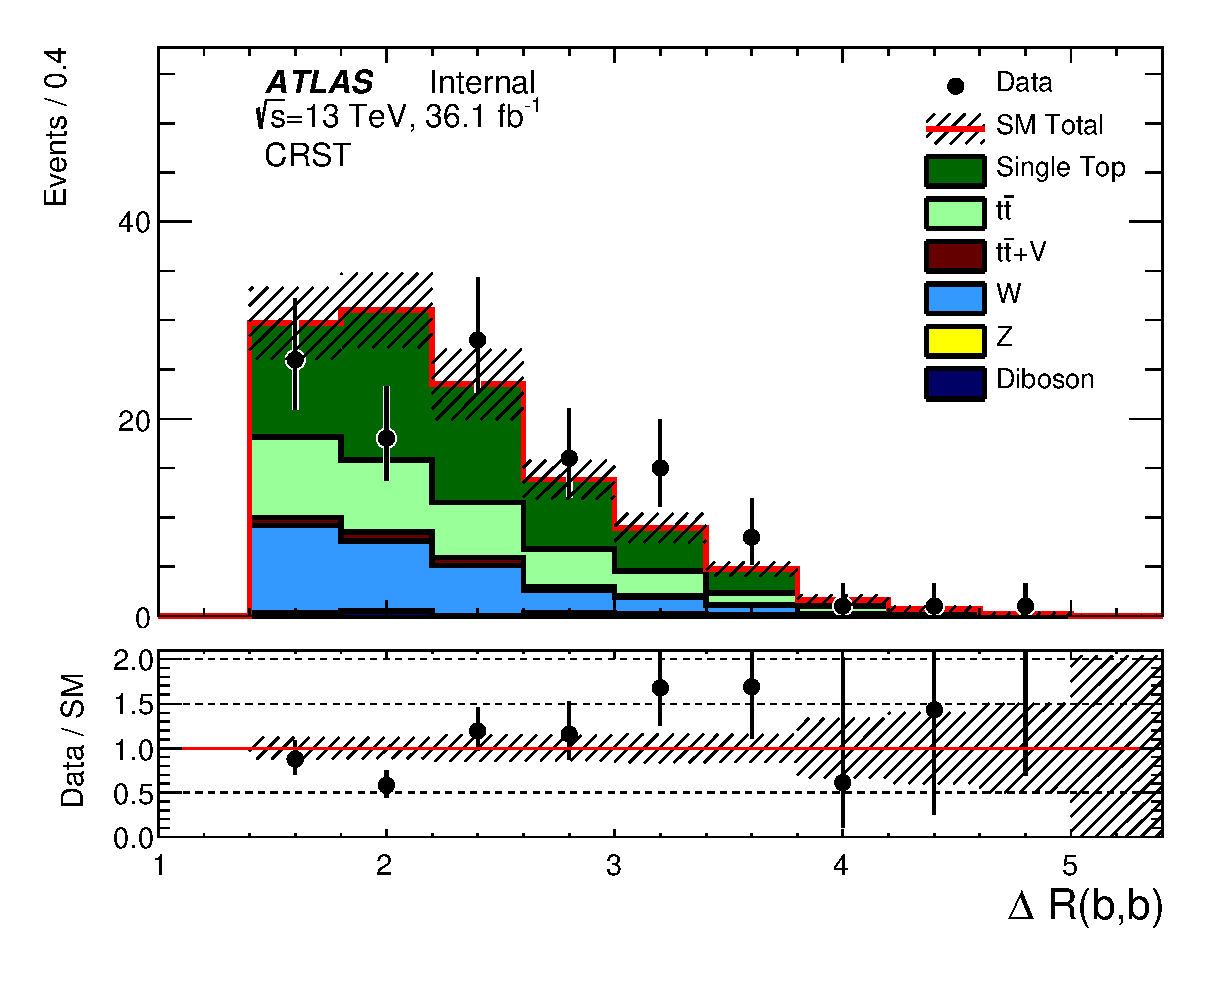
\includegraphics[width=0.45\textwidth]{figures/singleTop/postfit/DRBB_CRST.eps}
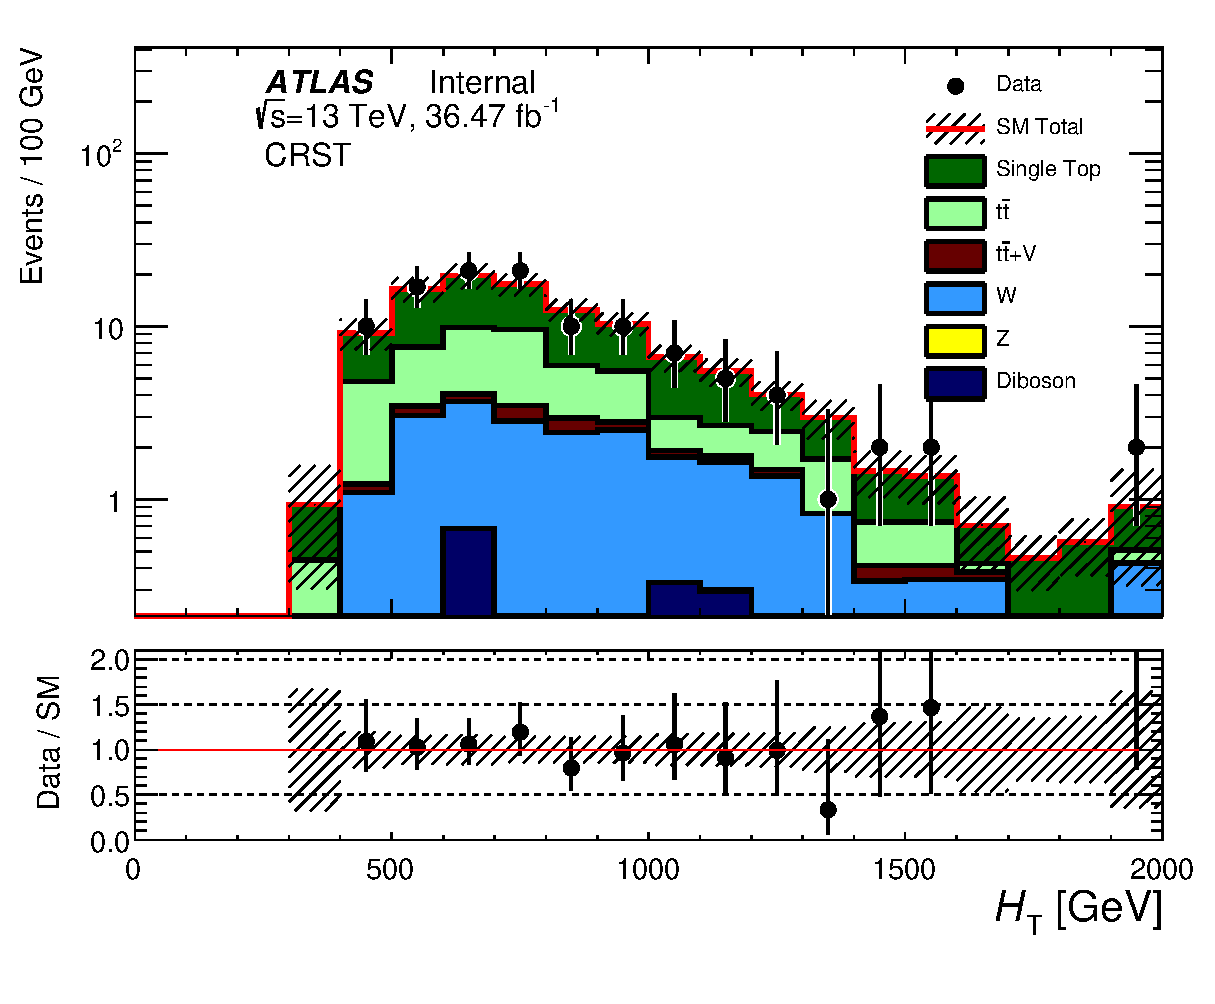
\includegraphics[width=0.45\textwidth]{figures/singleTop/postfit/Ht_CRST_log.eps}
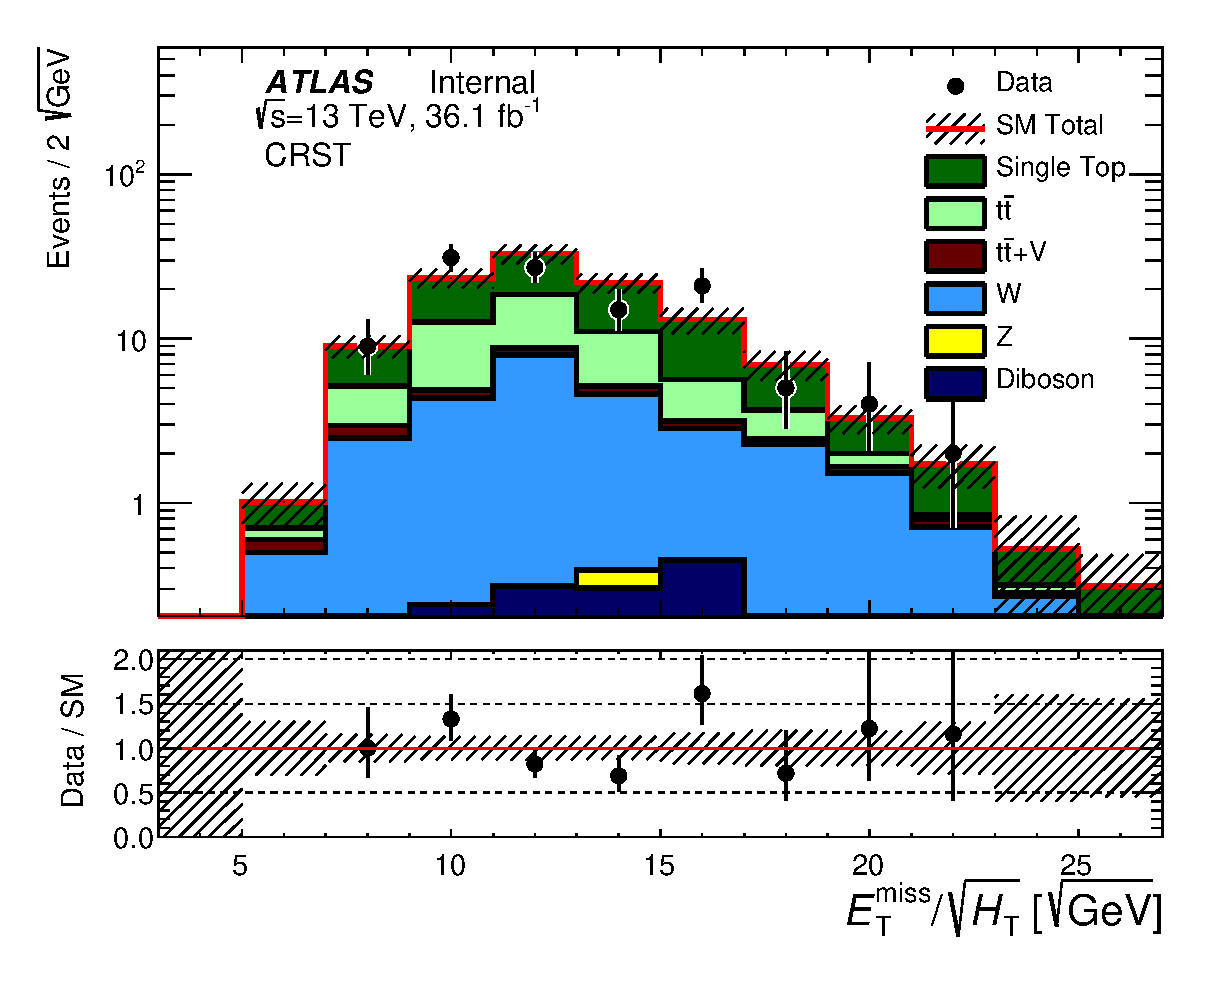
\includegraphics[width=0.45\textwidth]{figures/singleTop/postfit/HtSig_CRST_log.eps}
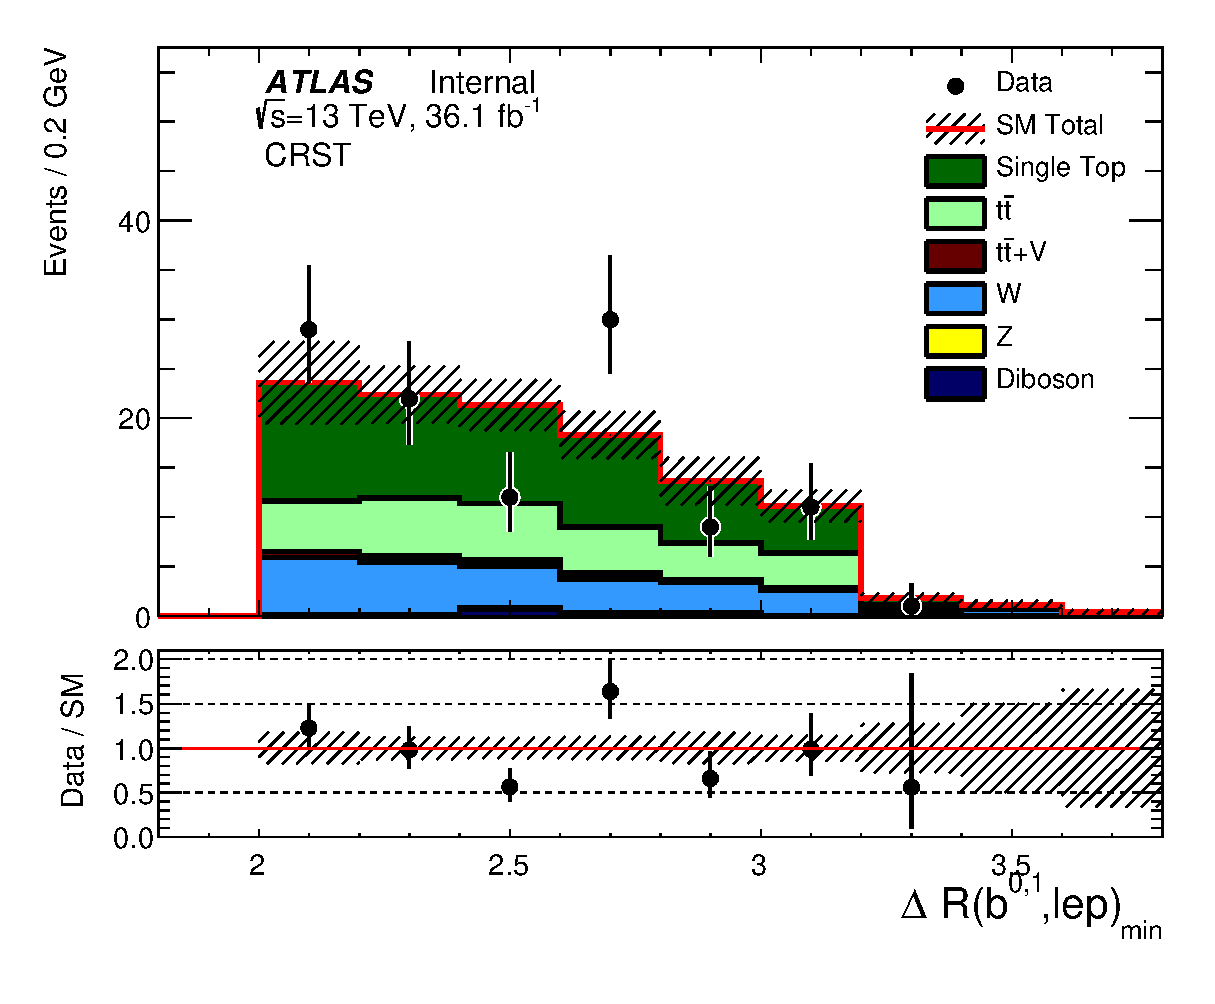
\includegraphics[width=0.45\textwidth]{figures/singleTop/postfit/MinDRBLep_CRST.eps}
\end{center}
\caption{Single top postfit control region distributions for \intlumi\ \ifb\ of data. The ratio between data and MC is shown in the bottom panel. The hashed area in both the top and lower panel represent the uncertainty due to MC statistics.}
\label{fig:CRST}
\end{figure}

\begin{figure}[htbp]
\begin{center}
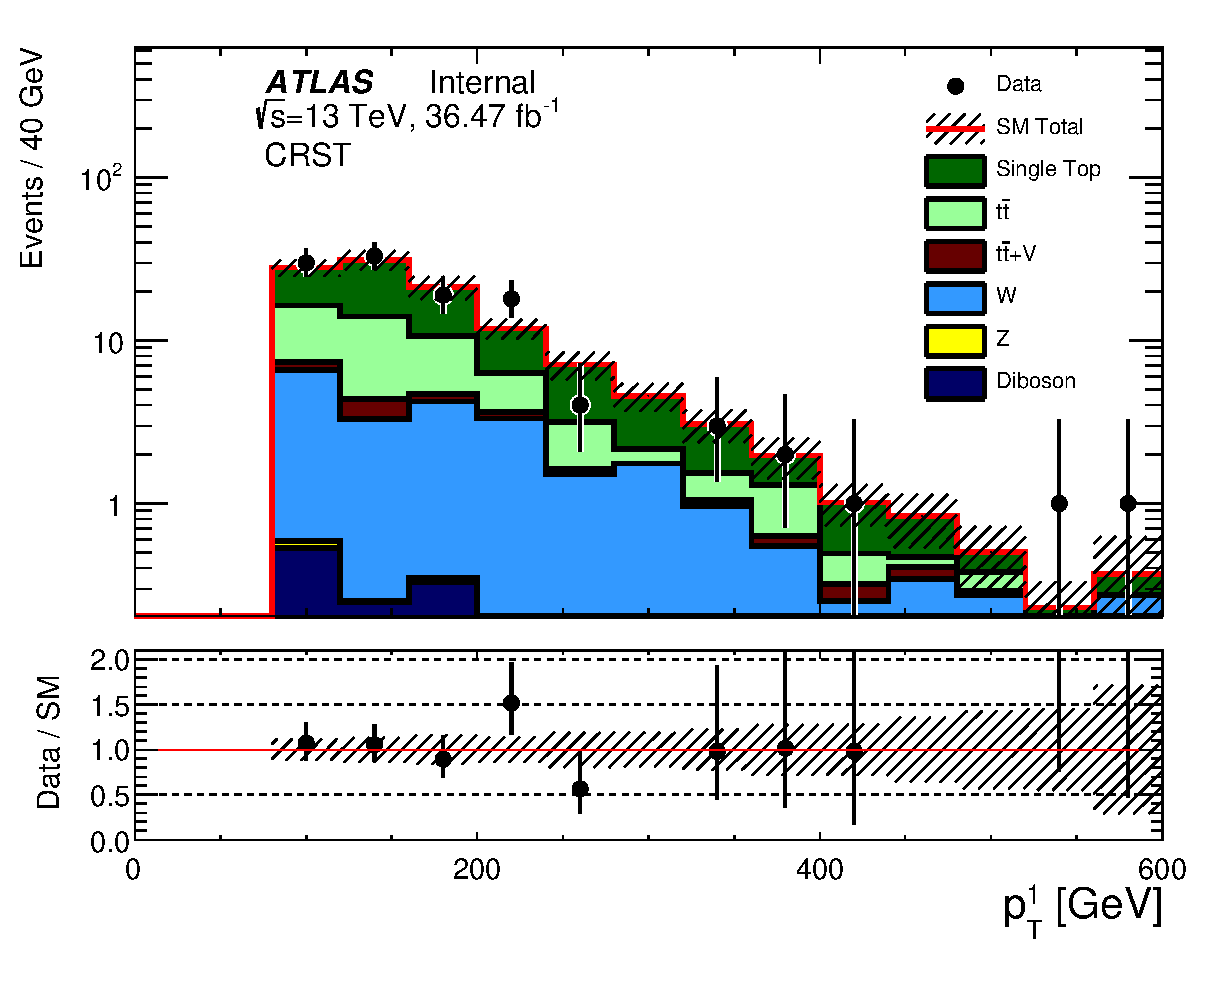
\includegraphics[width=0.45\textwidth]{figures/singleTop/postfit/JetPt_1__CRST_log.eps}
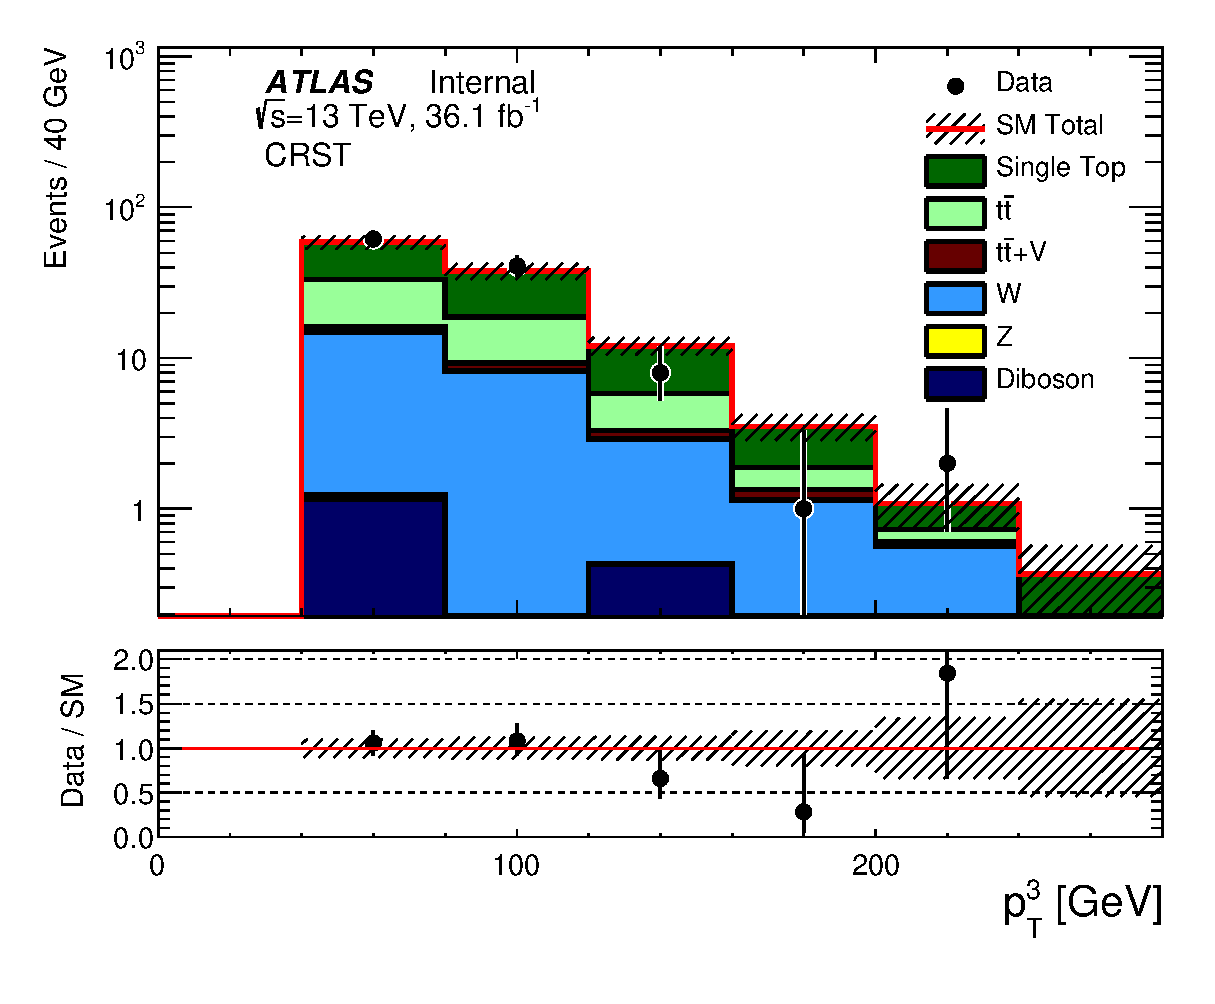
\includegraphics[width=0.45\textwidth]{figures/singleTop/postfit/JetPt_3__CRST_log.eps}
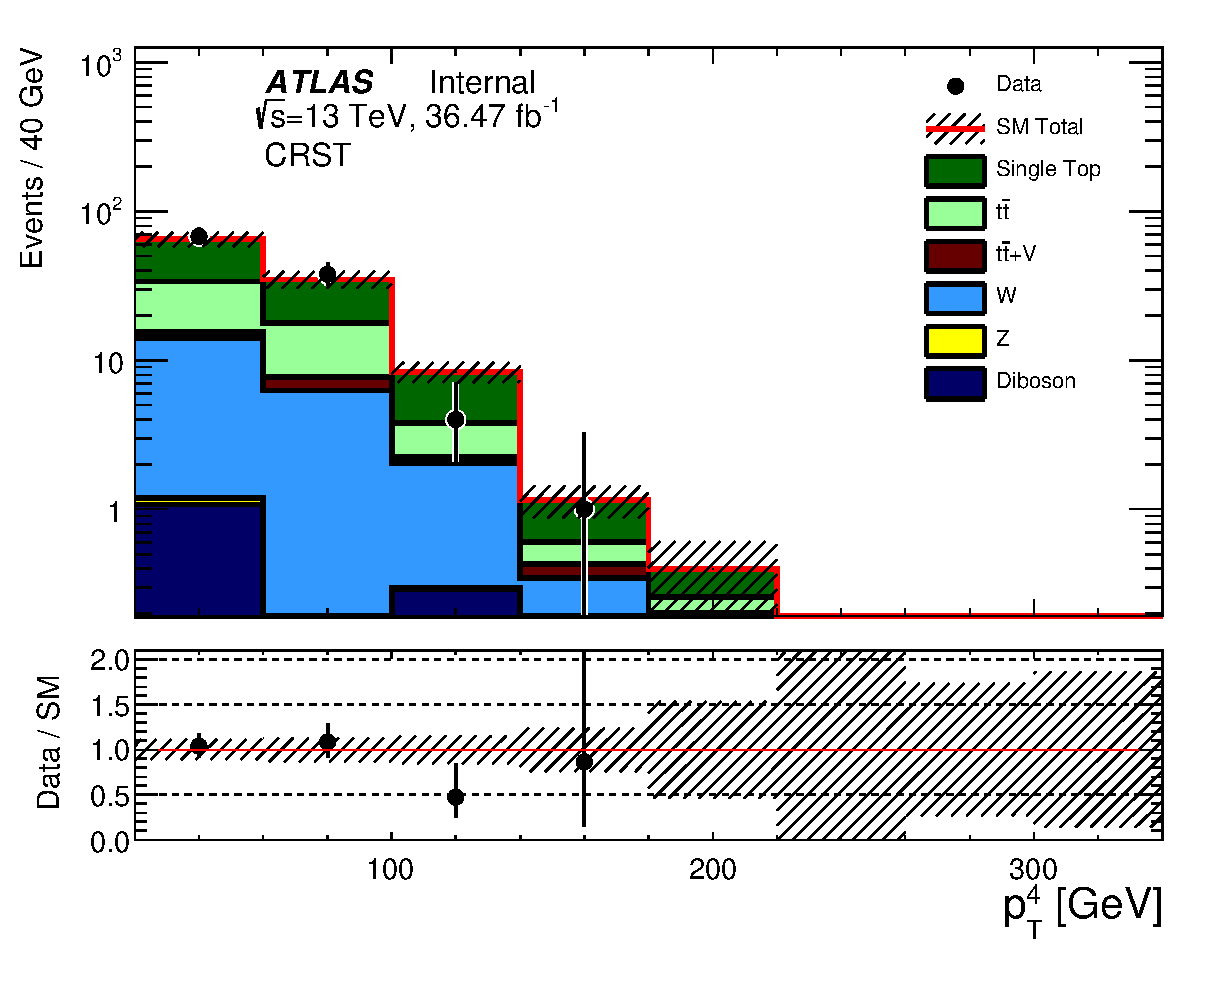
\includegraphics[width=0.45\textwidth]{figures/singleTop/postfit/JetPt_4__CRST_log.eps}
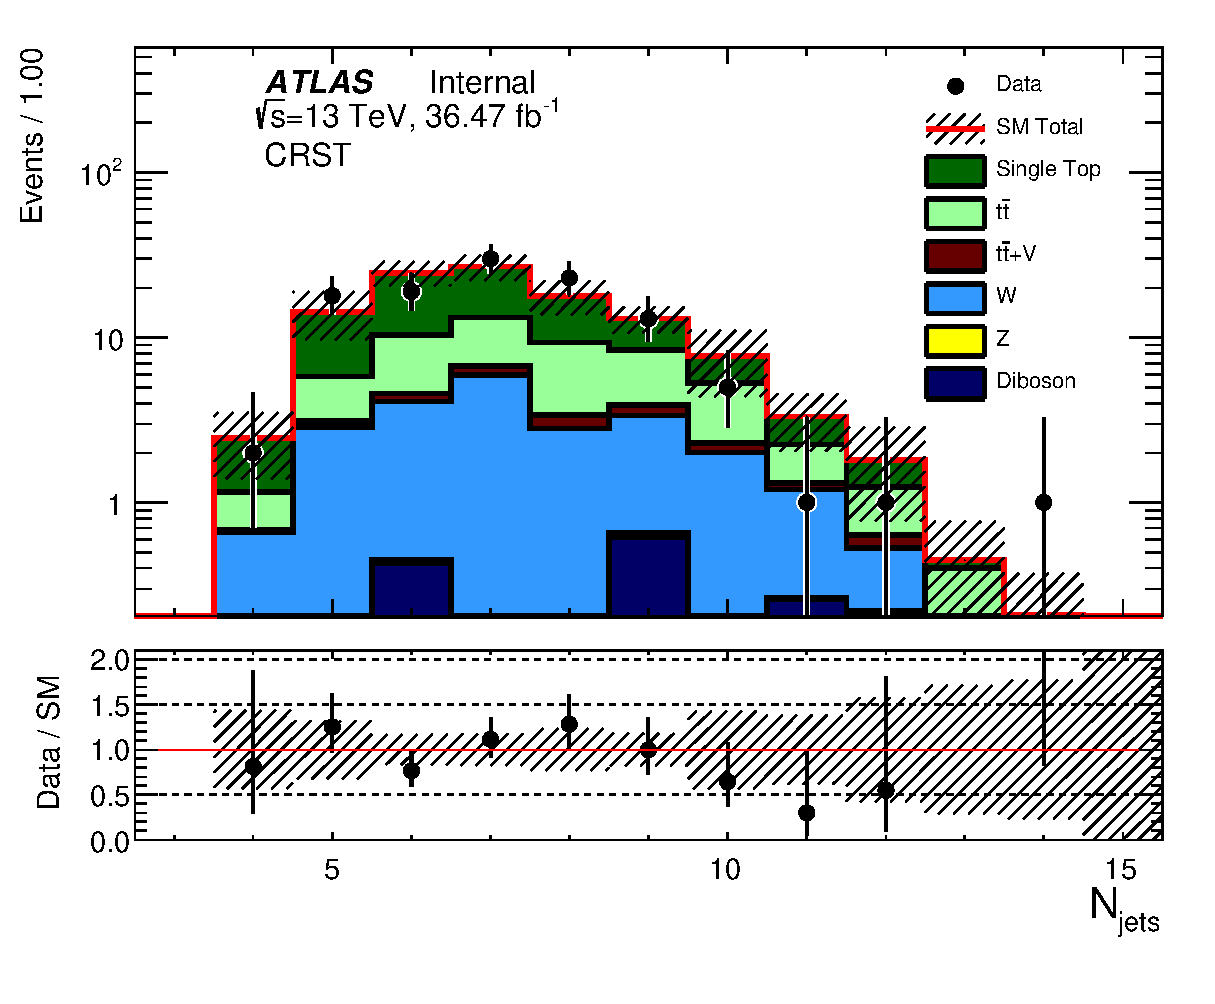
\includegraphics[width=0.45\textwidth]{figures/singleTop/postfit/NJets_CRST_log.eps}
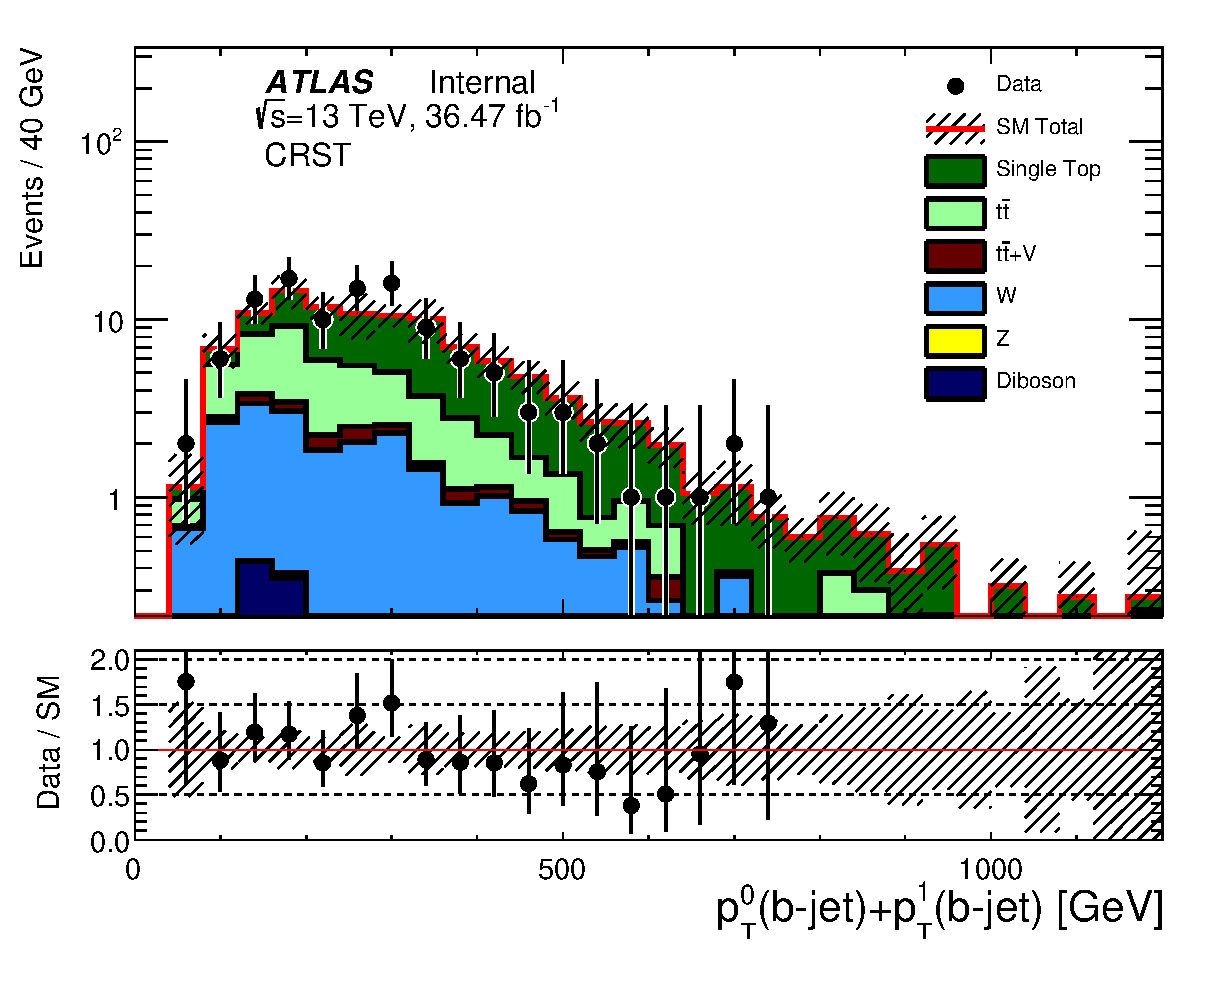
\includegraphics[width=0.45\textwidth]{figures/singleTop/postfit/JetPt_JetLeadTagIndex_JetPt_JetSubleadTagIndex__CRST_log.eps}

\end{center}
\caption{Single top postfit control region distributions for \intlumi\ \ifb\ of data. The ratio between data and MC is shown in the bottom panel. The hashed area in both the top and lower panel represent the uncertainty due to MC statistics.}
\label{fig:CRSTPTs}
\end{figure}

\begin{figure}[htbp]
\begin{center}
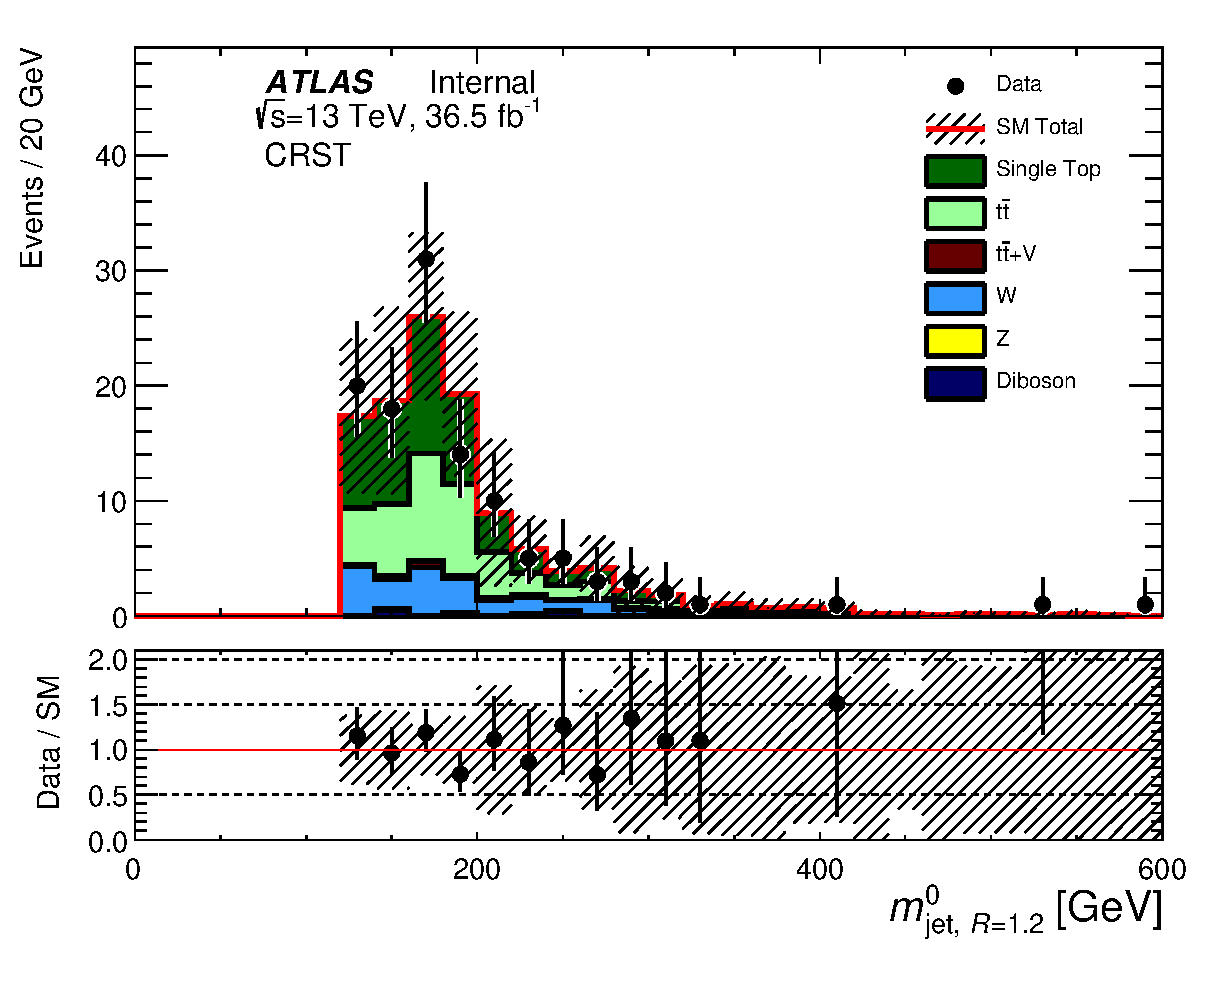
\includegraphics[width=0.45\textwidth]{figures/singleTop/postfit/AntiKt12M_0__CRST.eps}
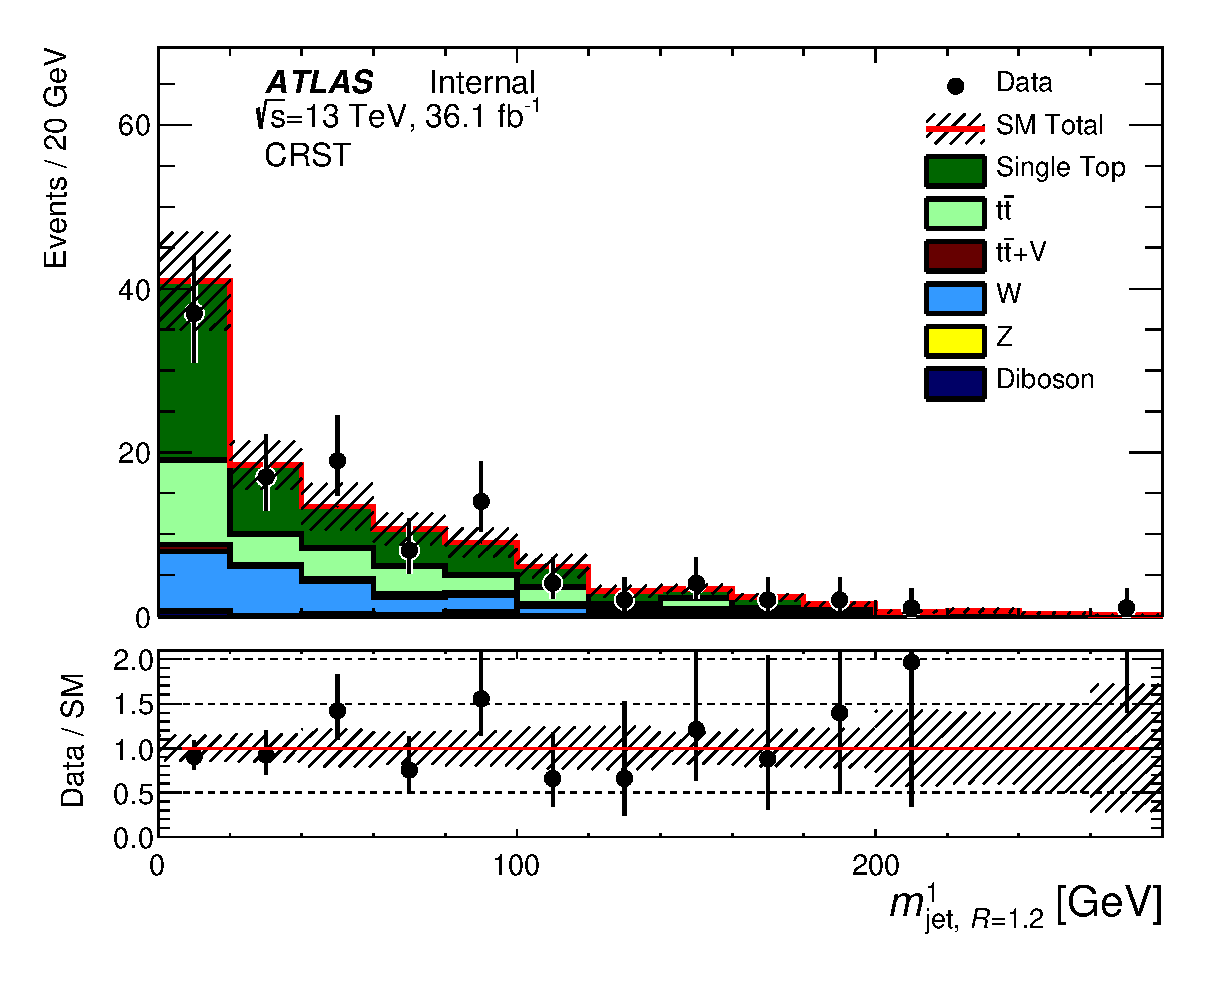
\includegraphics[width=0.45\textwidth]{figures/singleTop/postfit/AntiKt12M_1__CRST.eps}
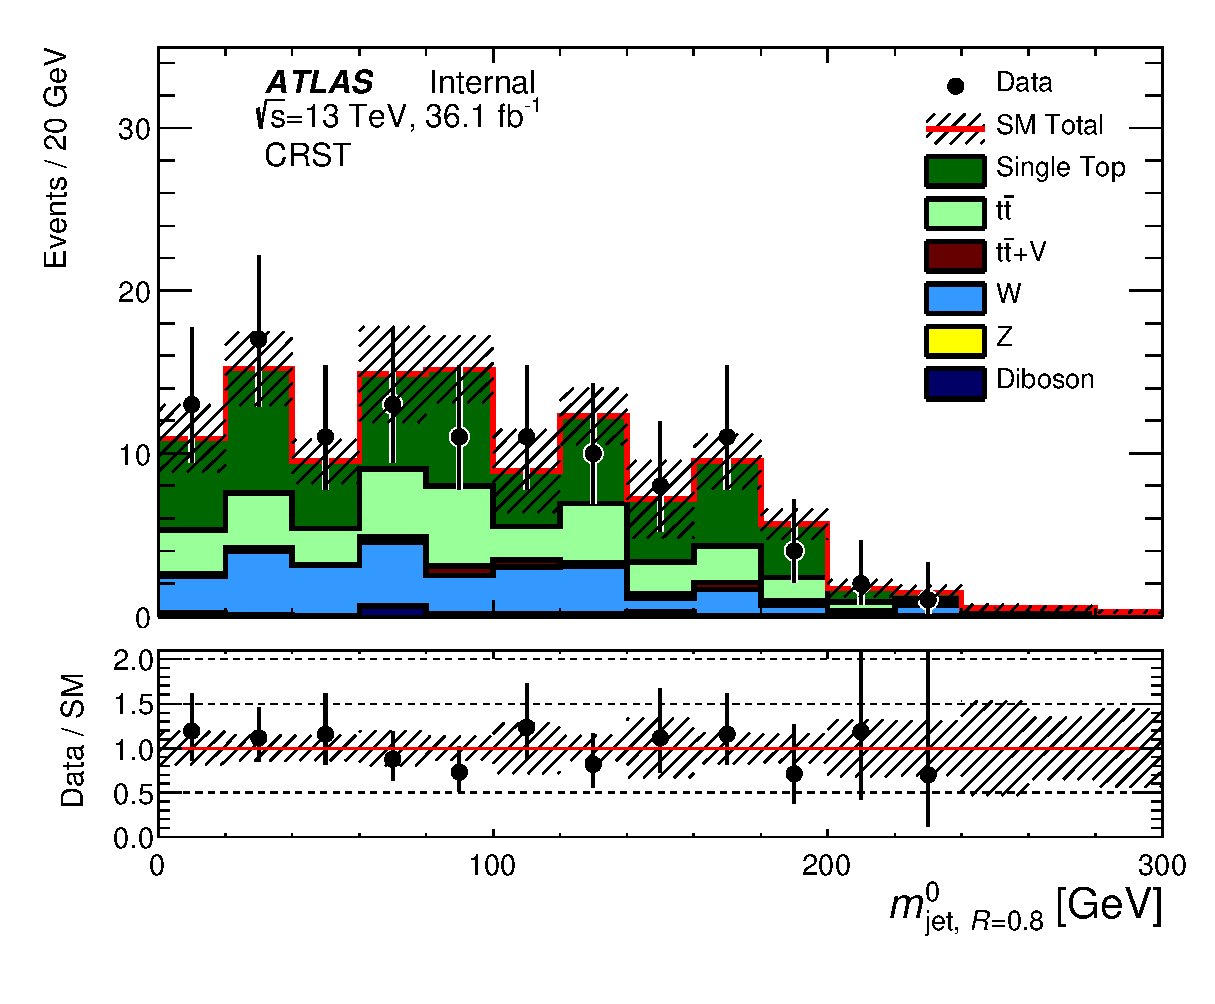
\includegraphics[width=0.45\textwidth]{figures/singleTop/postfit/AntiKt8M_0__CRST.eps}
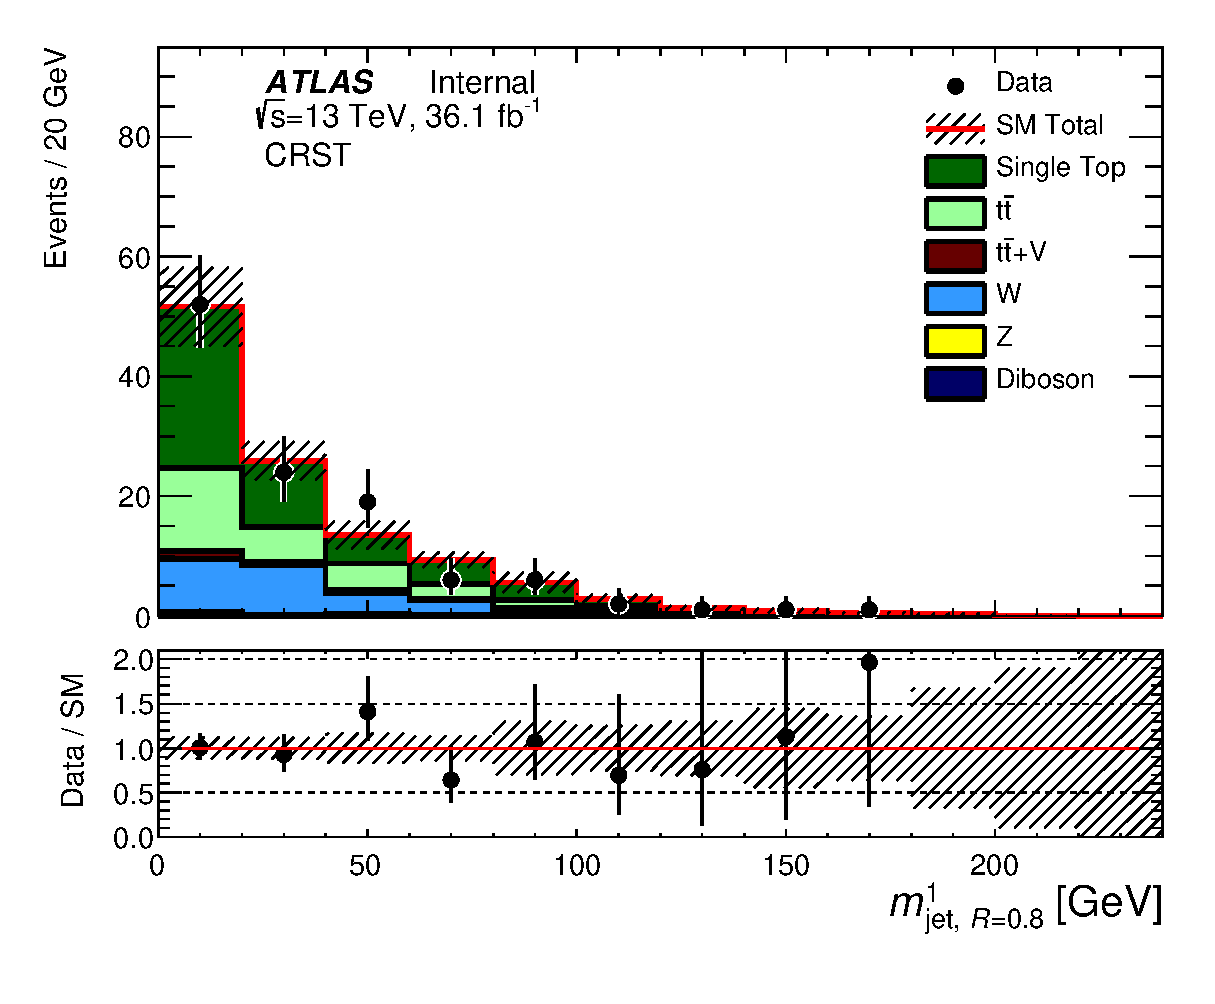
\includegraphics[width=0.45\textwidth]{figures/singleTop/postfit/AntiKt8M_1__CRST.eps}

\end{center}
\caption{Single top postfit control region distributions for \intlumi\ \ifb\ of data. The ratio between data and MC is shown in the bottom panel. The hashed area in both the top and lower panel represent the uncertainty due to MC statistics.}
\label{fig:CRSTMasses}
\end{figure}




\clearpage